\chapter{Wstęp}

Logistic regression — 1958 

Hidden Markov Model — 1960 

Stochastic gradient descent — 1960 

Support Vector Machine — 1963 

k-nearest neighbors — 1967 

Artificial Neural Networks — 1975 

Expectation Maximization — 1977 

Decision tree — 1986 

Q-learning — 1989 

Random forest — 1995 

4\% badań dotyczy oceny postępu w leczeniu [NVIDIA]

\begin{figure}[h!]
	\centering
	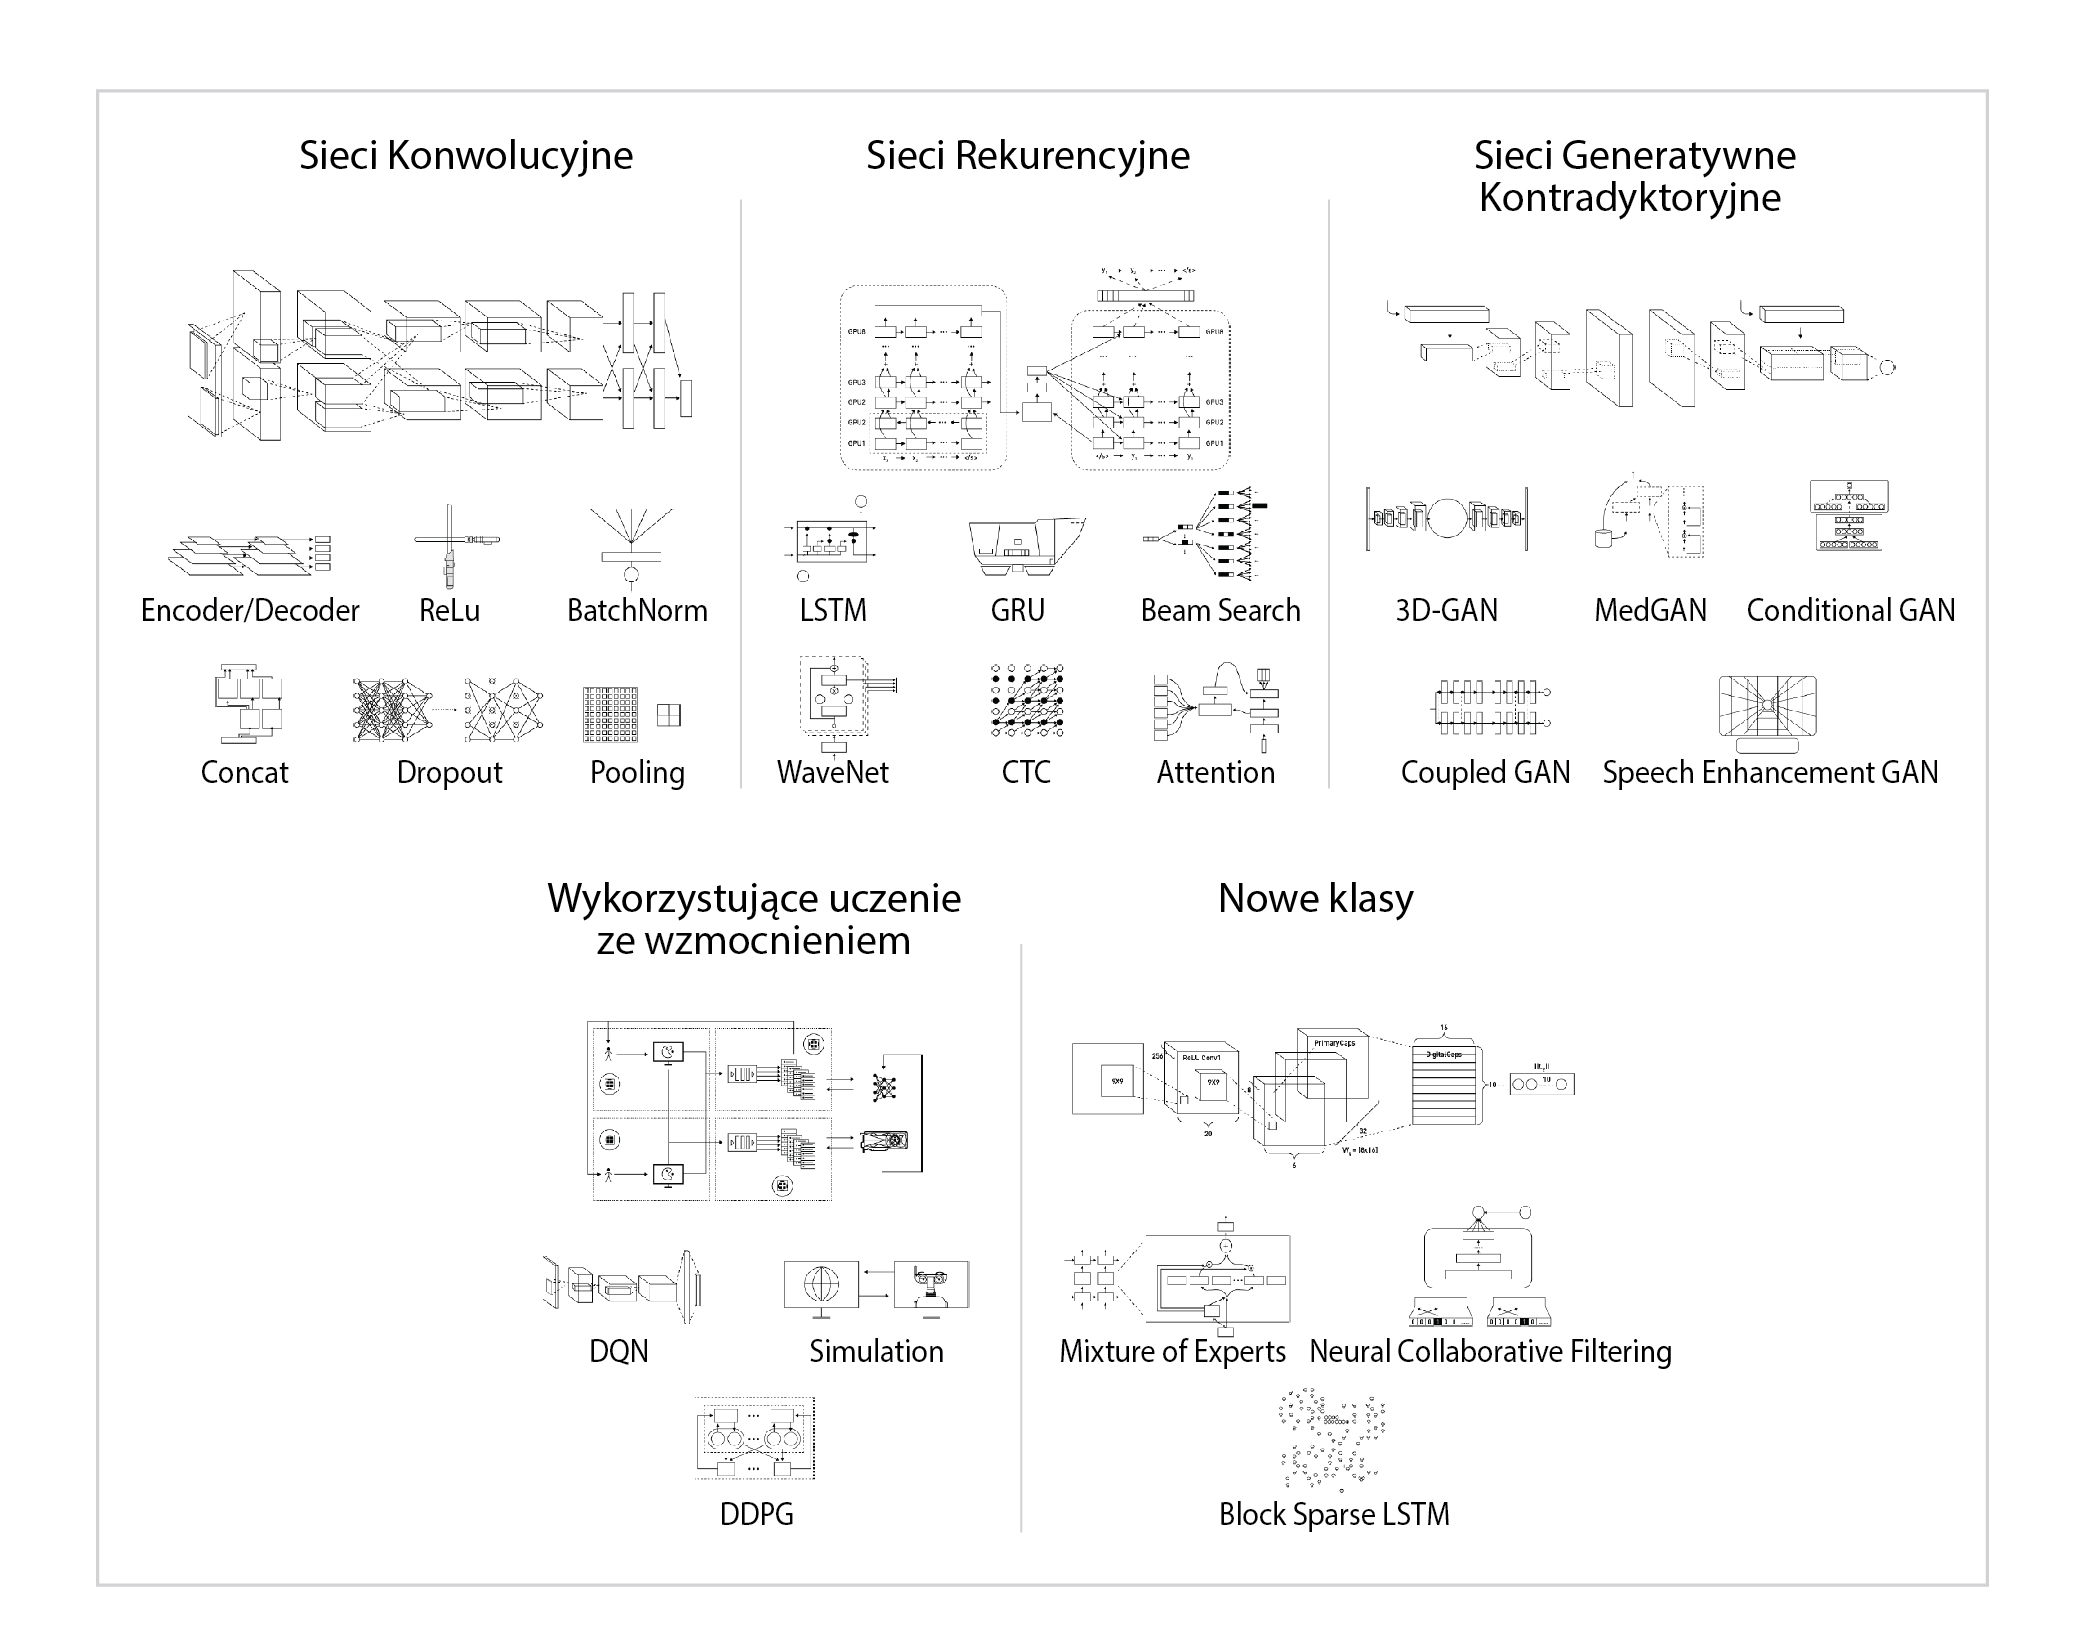
\includegraphics[width=1.0\textwidth]{figures/rodzajeSieciNeuronowych.png}
	\caption{Podział przedstawiający różne rodzaje współczesnych głębokich sieci neuronowych.}
	\label{DLcambrianExplosion}
\end{figure}
\chapter{Cel i przebieg pracy}




